%L'introduction est une section requise dans un rapport technique. Introduisez votre travail, l'idée de départ et les objectifs attendus. Un lecteur qui découvrirait votre projet au travers de cette introduction devrait ainsi être capable d'en comprendre le cadre, l'idée générale et les aboutissants du projet.
Dans le cadre des études à la HEIG-VD, un travail de Bachelor et demandé en fin d'études. Ce dernier représente un projet sur un semestre. 

\section{Contexte}
%Cette section \underline{n'est pas obligatoire}, mais elle est souvent présente dans un rapport technique pour compléter l'introduction et définir le contexte du travail \cad le cadre formel dans lequel le travail est mené.
Dans le domaine de la santé, les nouveau-nés sont des patients requérant une attention particulière et un contrôle précis de leurs 
paramètres vitaux. En effet, dès leur plus jeune âge, ils peuvent être victimes de plusieurs maladies dont les détresses respiratoires. 
De ce fait, plusieurs appareils de monitoring sont utilisés afin de contrôler, par exemple, l'activité pulmonaire des patients. 
Selon le type de patient, les appareils utilisés sont différents. En effet, un nouveau-né a un comportement différent d'une personne 
adulte. Il est alors nécessaire de contrôler ces paramètres vitaux à l'aide d'appareils adaptés. \\

Ce Travail de Bachelor porte sur la faisabilité d'un débitmètre respiratoire par nanotechnologie. Ce dernier permettrait de calculer le flux 
d'air entrant et sortant du patient avec des performances meilleures que ce qui existe actuellement sur le marché. \\

L'objectif principal de ce projet est donc de fabriquer des débitmètres par nanotechnologie ainsi qu'un banc de test adapté permettant de tester le 
fonctionnement de ces nouveaux capteurs. 

\section{Objectifs spécifiques}
Le cahier des charges complet est accessible dans les annexes. Ce chapitre se concentrera sur les différents objectifs compris dans le cahier 
des charges. \\
\begin{itemize}
    \item Élaboration d'un cahier de spécifications \& élaboration d'un catalogue de solutions
    \item Conception et réalisation d'un débitmètre par nanotechnologie
    \item Montage d'un banc de test dédié au débitmètre
    \item Qualification des performances du débitmètre
\end{itemize}

\section{État de l'art}
\subsection{Débitmètres néonatals sur le marché}
\begin{comment}
Actuellement, ce qui existe sur le marché sont des anémomètres à double fils chauds (double hot wire anemometer). Ces débitmètres 
mesurent le flux des patients néonatals. \\
Les revues scientifiques parlent également de débitmètre pédiatrique. Leur fonctionnement  
\end{comment}
Plusieurs entreprises proposent des débitmètres néonatals. Ces entreprises ont été regroupées dans le tableau ci-dessous avec les 
technologies de capteur utilisées. \\

\begin{table}[H]
    \centering
    \begin{tabular}{|c|c|}
        \hline
        Entreprises & Technologie                         \\
        \hline
        Sensirion   & Capteur thermique de débit massique \\
        \hline
        Mim-Germany & Anémomètre à fil chaud double       \\
        \hline
        Europlaz    &                                     \\
        \hline
        Draeger     & Anémomètre à fil chaud              \\
        \hline
    \end{tabular}
    \caption{Débitmètres pédiatriques sur le marché}
    \label{tab:debitmetreMarche}
\end{table}


\subsection{Revues scientifiques}
Les revues scientifiques sont également des ressources intéressantes à considérer pour l'élaboration de l'état de l'art. En effet, les 
articles scientifiques vont permettre d'établir une liste des techniques déjà exploitées, leur fonctionnement détaillé ainsi que leurs 
performances. \\
\begin{figure}[H]
    \hspace{-1cm}
    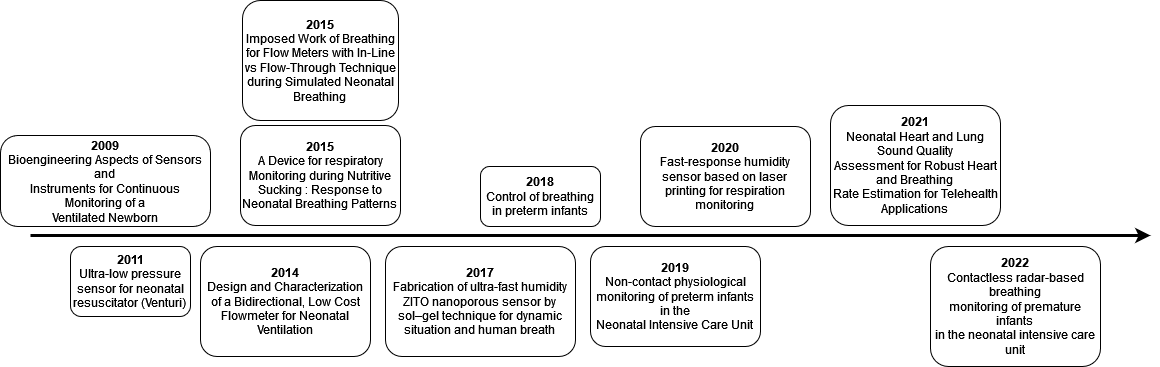
\includegraphics[scale = 0.45]{images/DRP_Etat_de_l_art.png}
    \caption{Articles scientifiques par ordre chronologique}
    \label{fig:articlesChrono}
\end{figure}

Les articles pertinents pour ce Travail de Bachelor sont résumés dans ce chapitre et classé par ordre chronologique sur la figure 
\ref{fig:articlesChrono}. 

\subsubsection{Effet de Venturi}
Le débit respiratoire est mesuré grâce à une différence de pression. Cette différence de pression est engendré par un rétrécissement de 
l'espace de circulation du gaz (principe de Venturi) \cite{oberg_biomedical_2011}. 
\begin{figure}[H]
    \centering
    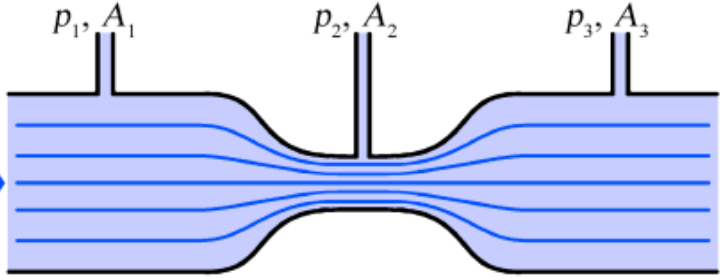
\includegraphics[scale = 0.5]{assets/figures/Venturi.png}
    \caption{Effet de Venturi \cite{oberg_biomedical_2011}}
    \label{fig:venturi}
\end{figure}

La figure \ref{fig:venturi} illustre l'effet Venturi. Avec un rétrécissement de la partie centrale d'un tube, le fluide traversant le dispositif 
sera accéléré et subira également une dépression à cet endroit. Ainsi, en mesurant la pression à différents endroits du tube, il est possible 
de calculer le flux d'air. \\

C'est la technologie utilisée par les pneumotachographes (le pneumotacographe de Fleisch par exemple). Mais elle peut également être utilisée 
dans une application quelque peu différente. En effet, un article mentionne son utilisation dans un ressuscitateur \cite{jacq_ultra-low_2011}. 
Un tel appareil permet la réanimation du patient qui ne respire plus. Le ressuscitateur gonfle les poumons d'air et ainsi s'assure qu'un bon 
taux d'oxygène circule dans le patient. \\
Pour les nouveaux-né, la quantité d'air injectée dans les poumons doit être mesurée, car un trop grand débit pourrait rapidement engendrer 
des dégâts. \\
Couplé au système de Venturi, un capteur de force vient mesurer la pression et le volume d'air passant par le ressuscitateur. 

\subsubsection{Anémomètre à fils chauds}
Par la suite, il est expliqué que le pneumotachographe est gentiment remplacé par les anémomètres à fil chaud. Ces capteurs sont 
constitués d'un ou plusieurs fils chauffés par une source de courant. Lorsqu'un flux d'air va souffler sur le fil, la chaleur sera 
transférée du fil au gaz. Le capteur viendra alors mesurer la quantité de chaleur transférée ainsi que la différence de température entre 
le fil et le gaz pour finalement calculer le débit \cite{oberg_biomedical_2011}. \\
L'article susmentionné conseil l'utilisation des anémomètres à plusieurs fils contrairement à ceux à un seul fil qui aurait des performances 
moindres. 
L'anémomètre à fils chauds est une technologie incorporée par exemple dans la machine "Draeger Babylog", marque mentionnée dans le tableau \ref{tab:debitmetreMarche}. 

\subsubsection{Transfert de chaleur entre deux transistors}

Une autre technologie pour débitmètre consiste à utiliser le transfert de chaleur entre deux transistors. 
\begin{figure}[H]
    \centering
    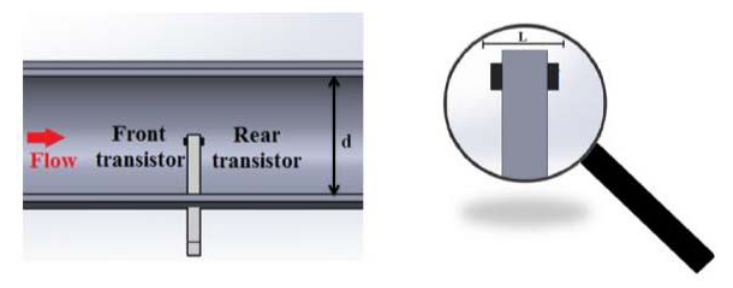
\includegraphics[scale = 0.5]{images/Debitmetre_transistors.png}
    \caption{Principe du débitmètre à transistors}
    \label{fig:transistors}
\end{figure}

C'est un principe encore innovant décrit dans l'article \cite{giorgino_design_2014}, utilisé dans l'article \cite{rosi_device_2016} et illustré 
par la figure \ref{fig:transistors}. 
Le premier transistor (appelé Front transistor) est placé perpendiculairement au flux d'air sur un PCB. \\
Le second (Rear transistor) est fixé de l'autre côté du PCB dos à dos avec le premier transistor (cf. figure \ref{fig:transistors}). \\
De cette manière, le capteur sera capable de distinguer une expiration d'une inspiration. Le temps de réponse d'un tel capteur serait 
d'environ 340 ms. C'est un très bon temps de réponse en comparaison des capteurs médicaux existants sur le marché. Cependant, diverses améliorations 
doivent encore être faites avant de pouvoir utiliser une telle technologie. 

\begin{comment}
L'article suivant est intéressant au niveau du listage des débitmètres pédiatriques existants \cite{}. En effet, il étudie les différents fonctionnements 
existants et compare les signaux obtenus. Étant donné que cet article étudie plus précisément une caractéristique ("IN-line" vs "Flow-Through"), 
il est moins important dans le cadre de ce projet.\\
\end{comment}

\subsubsection{Caméra}
La thématique de l'article \cite{villarroel_non-contact_2019} repose sur une technologie de monitoring non invasive. Elle utilise une caméra qui suit les mouvements du nouveaux-né. 
Cette technologie permet également d'enregistrer d'autres signaux tels que la fréquence cardiaque, mais elle requiert encore quelques améliorations 
ainsi que quelques recherches supplémentaires. 

\subsubsection{Nanotechnologie}
Un autre article mentionne les membranes nanoporeuses comme capteur \cite{moharamzadeh_fabrication_2018}. Bien que cette technique se rapproche 
de notre application, ces capteurs sont pour l'humidité et non le débit respiratoire. Des nanostructures d'oxyde de Zinc sont utilisées, car 
elles possèdent de bonnes propriétés physiques et chimiques. Étant donné que l'humidité et le débit respiratoire sont en lien, l'article évoque 
également le débit, cependant, il ne l'étudie pas plus en détail. \\
Toutefois, un temps de réponse plutôt bon, de l'ordre de la seconde est attendu avec une telle technologie. 

\section{Benchmarking}
Avec les différentes informations récoltées de l'état de l'art, un benchmarking peut être élaboré. Ce dernier est composé de différentes valeurs 
de performance à atteindre dans l'idéal. 

\begin{table}[H]
    \centering
    \begin{tabular}{|c|c|}
        \hline
        \textbf{Plage de débit}           & $\pm 8$ l/min     \\
        \hline
        \textbf{Sensibilité de détection} & < 0.1 l/min       \\
        \hline
        \textbf{Temps de réponse}         & < 340 ms          \\
        \hline
        \textbf{Fréquence de respiration} & entre 0.3 et 3 Hz \\
        \hline
        \textbf{Géométrie des conduits}   & < 10 mm           \\
        \hline
    \end{tabular}
    \caption{Benchmarking}
    \label{fig:benchmarking}
\end{table}


\section{Fonctionnement du débitmètre respiratoire pédiatrique}
Ce travail de Bachelor est donc une recherche à propos d'un débitmètre dont le principe de fonctionnement est encore innovant. \\

Le capteur développé repose sur le phénomène de l'effet Seebeck, phénomène que l'on peut également retrouver dans les thermocouples. L'effet 
Seebeck est le suivant :\\
Lorsque deux matériaux conducteurs ou semi-conducteurs sont soumis à des températures différentes, une tension va être produite entre ces deux matériaux. \\
Sur la Figure \ref{fig:Seebeck}, deux matériaux sont côte à côte. Une source de chaleur vient chauffer le matériau de gauche. 
\begin{figure}[H]
    \centering
    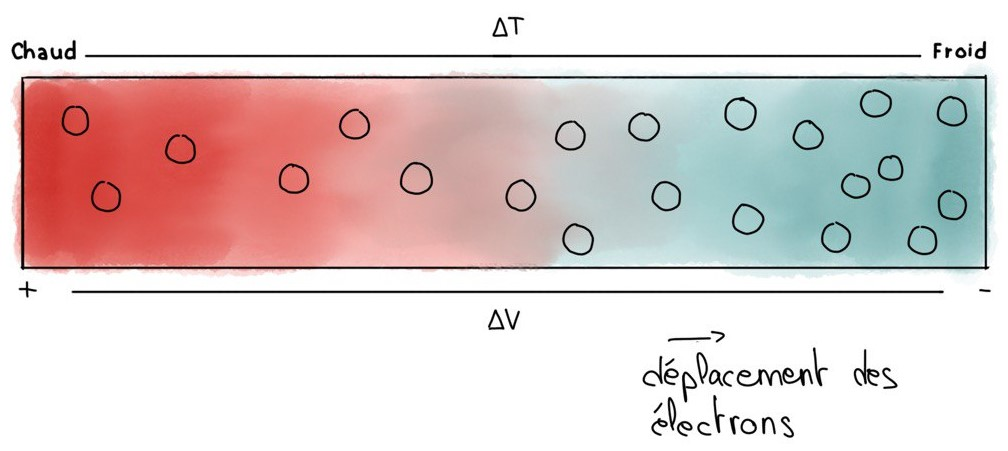
\includegraphics[scale = 0.3]{images/Seebeck.jpg}
    \caption{Effet de Seebeck}
    \label{fig:Seebeck}
\end{figure}
Les électrons au sein de la matière vont se déplacer du chaud vers le froid, créant ainsi un courant \cite{instrumentys_effet_2021}.\\
La tension est calculée grâce à la formule suivante :
\[V = S \cdot (T_{chaude} - T_{froide})\]
Avec S, le coefficient de Seebeck\\

Comme évoqué plus haut, le capteur est constitué de membranes nanoporeuses achetées sur le marché. 
Un côté de la membrane va être recouvert d'un matériau conducteur, l'or, grâce à un dépôt physique en phase vapeur (\gls{pvd}). Puis, Les pores de cette membrane sont remplies par 
électrodéposition (\gls{ed}) avec une solution de Tellure de Bismuth ou $Bi_2Te_3$ (cf. figure \ref{fig:electrodeposition}). Ces pores remplis de tellure de 
Bismuth deviennent alors des nanofils. 
\begin{figure}[H]
    \centering
    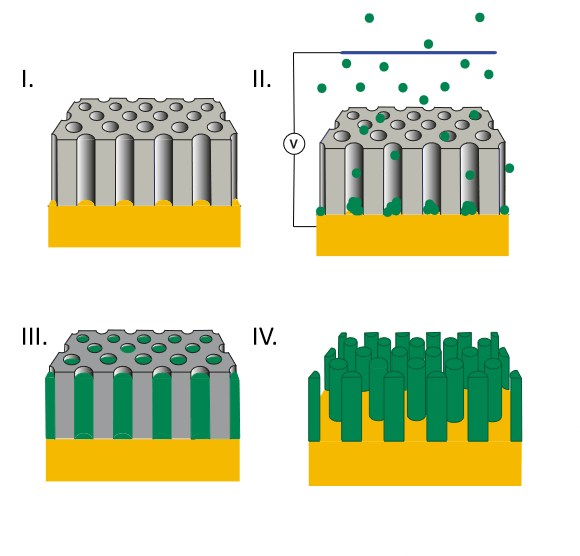
\includegraphics[scale = 0.4]{images/Electrodeposition.png}
    \caption{Électrodéposition}
    \label{fig:electrodeposition}
\end{figure}

Le fonctionnement du débitmètre pédiatrique combine la nanotechnologie et l'effet de Seebeck. \\
En effet, un corps de chauffe est placé entre deux couches d'or en forme de L (cf. figure \ref{fig:schema_global}). Lorsqu'un courant viendra 
alimenter la piste d'or du milieu, celle-ci va s'échauffer. Une différence de température va se créer entre les deux pistes d'or en "L" lorsque 
le patient viendra expirer ou inspirer de l'air sur le corps de chauffe (figure \ref{fig:schema_coupe}). 
\begin{figure}[H]
    \centering
    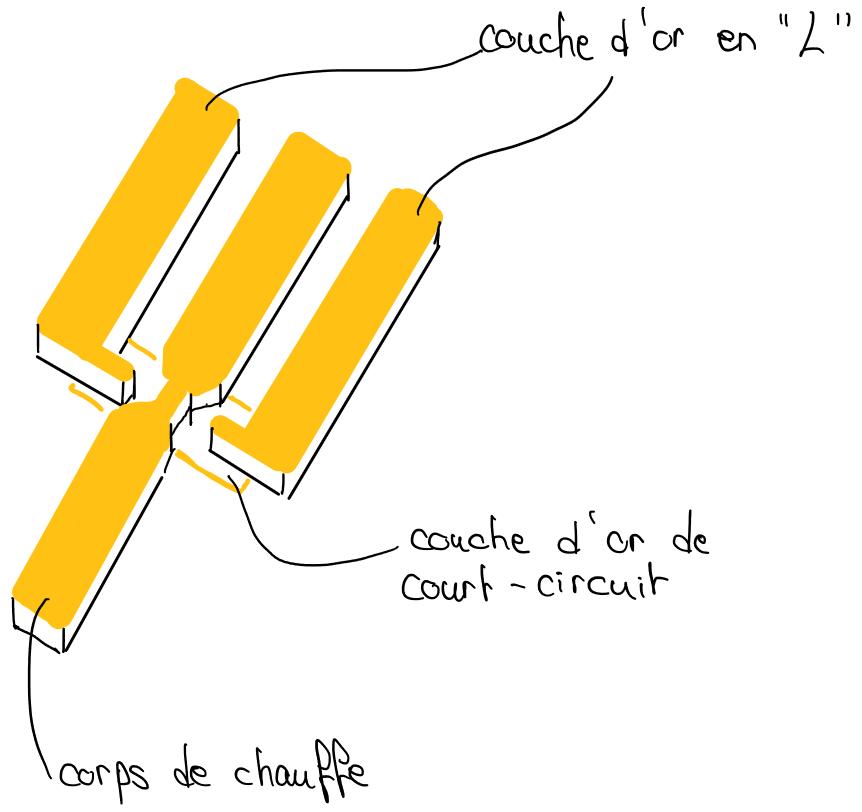
\includegraphics[scale = 0.4]{assets/figures/schema_capteur_vue_generale.png}
    \caption{Schéma du capteur - Vue globale}
    \label{fig:schema_global}
\end{figure}
\begin{figure}[H]
    \hspace{-0.7cm}
    \begin{subfigure}{0.4\textwidth}
        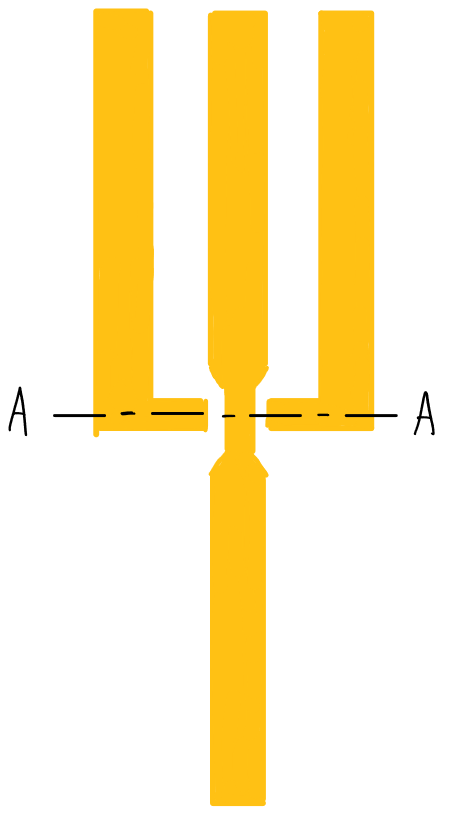
\includegraphics[scale = 0.3]{assets/figures/schema_capteur_vue_dessus.png}
        \caption{Schéma du capteur - Vue de dessus}
        \label{fig:schema_dessus}
    \end{subfigure}
    \begin{subfigure}{0.4\textwidth}
        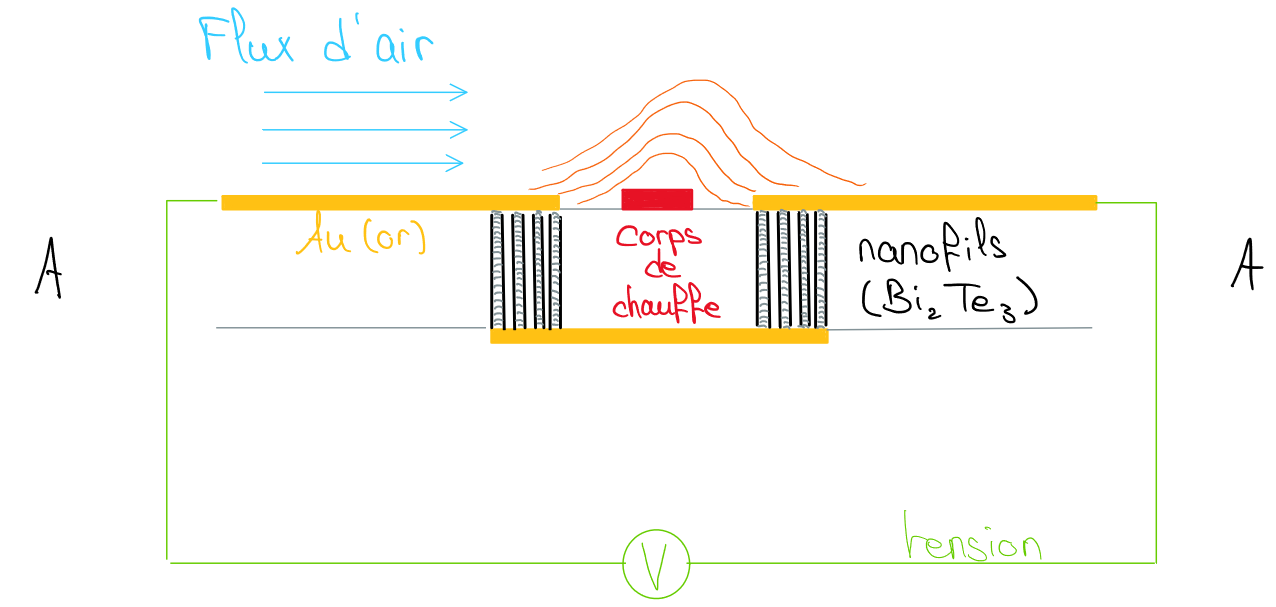
\includegraphics[scale = 0.4]{images/CapteurFUN.png}
        \caption{Schéma du capteur - Vue en coupe}
        \label{fig:schema_coupe}
    \end{subfigure}
    \caption{Schéma du capteur - Vue de dessus et en coupe}
\end{figure}
Nous pouvons observer sur la figure \ref{fig:schema_coupe} que plusieurs électrodépositions (\gls{ed}) sont faites (à l'endroit des nanofils). Une première 
se situe à gauche du corps de chauffe et la deuxième, à sa droite. \\
Avec une différence de température de part et d'autre du corps de chauffe, un courant va circuler entre la couche d'or en "L" de gauche, à 
travers les nanofils gauches, au sein de la couche d'or du bas (couche d'or de court-circuit) puis dans les nanofils de droite (circuit du thermoélectrique). 
Une tension va apparaître et il sera alors possible de lier cette tension au débit inspiré et expiré du nouveau-né.\\
Cette membrane nanoporeuse associée des différentes électrodépositions et couches d'or sera appelée capteur \gls{capteur}. 

Étant donné que les nanopores sont extrêmement fins et courts, il est attendu d'obtenir un temps de réponse très intéressant (temps 
de réponse faible). 

\section{Livrables}
\begin{itemize}
    \item Cahier de spécifications
    \item Débitmètre fonctionnel
    \item Banc de test
    \item Rapport technique
\end{itemize}
\section{Planification}
Image\\

L'avancée du travail a été suivie par une séance d'une heure hebdomadaire. 

\section{Plan du rapport}
Le travail effectué s'est organisé en plusieurs parties : \\
\begin{enumerate}
    \item Cahier des spécifications\\
          Revue de la littérature, rédaction d'un état de l'art et définition du benchmarking. \\
    \item Conception et réalisation du capteur nanostructuré\\
          Électrodéposition, déposition physique en phase vapeur (\gls{pvd}), conditionnement du capteur (réalisation des supports)\\
    \item Conception et réalisation du banc de test\\
          Commandes, études des différents composants du banc de test, réalisation, montage et validation\\
    \item Qualification du capteur\\
          Définition d'un protocole de mesures, résultats et analyses\\
    \item Rapport technique\\
          Rédaction du rapport
\end{enumerate}

\begin{comment}
%%if
\section{Citations et bibliographie}
Citer vos sources est essentiel. Avec \texttt{biblatex} vous pouvez facilement citer des articles, des livres ou des sites internet. Toutes les citations dans le texte seront automatiquement regroupées en fin de document dans la section \guillemotleft Bibliographie\guillemotright. Par exemple, citons un article d'Einstein \cite{einstein} ou le livre de Dirac \cite{dirac}.

Parfois, il peut être utile d'utiliser un gestionnaire de bibliographie. La communauté académique recommande l'outil \href{https://www.zotero.org/}{Zotero} qui permet de gérer une bibliothèque numérique d'ouvrages et de références numériques. Il permet également de générer une bibliographie compatible avec \LaTeX.

Notez qu'il est très facile d'obtenir l'extrait \texttt{bibtex} depuis des journaux. Sélectionnez \emph{export/citation}. Si vous le pouvez choisissez \texttt{bibtex}. Dans le cas d'un format \texttt{.ris}, utilisez un convertisseur en ligne comme \href{http://www.bruot.org/ris2bib/}{ris2bib}.

\section{Adapter votre modèle}
Ce document n'est qu'un modèle ayant pour but de revoir les quelques avantages de \LaTeX~ et les fonctionnalités qui pourraient vous être utiles pour rédiger un rapport académique. N'hésitez pas à supprimer les parties inutiles et à adapter ce modèle à vos besoins.
%%fi
\end{comment}